%%%%%%%%%%%%%%%%%%%%%%%%%%%%%%%%%%%%%%%%%%%%%%%%%%%%%%%%%%%%
%%  This Beamer template was created by Cameron Bracken.
%%  Anyone can freely use or modify it for any purpose
%%  without attribution.
%%
%%  The current presentation created by Jeferson L. R. Souza (jefecomp) is based on the template created by Cameron Bracken. 
%%  
%%  Small modifications have been introduced and anyone is free to use such modified version.
%%
%% Last Modified: June 14, 2015.

\documentclass[xcolor=x11names,compress]{beamer}

%% General document %%%%%%%%%%%%%%%%%%%%%%%%%%%%%%%%%%
\usepackage{graphicx}
\usepackage{tikz}
\usetikzlibrary{decorations.fractals}
%%%%%%%%%%%%%%%%%%%%%%%%%%%%%%%%%%%%%%%%%%%%%%%%%%%%%%

%Hyperref
\usepackage{hyperref}

%Multirow package
\usepackage{multirow} 

%Math packages
\usepackage{amsmath}
\usepackage{textcomp}


%% Beamer Layout %%%%%%%%%%%%%%%%%%%%%%%%%%%%%%%%%%
\useoutertheme[footline=authorinstitutetitle,subsection=false,shadow]{miniframes}
\useinnertheme{default}
\usefonttheme{professionalfonts}
\usepackage{mathpazo}

\setbeamerfont{title like}{shape=\scshape,series=\bfseries}
\setbeamerfont{frametitle}{shape=\scshape,series=\bfseries}

\setbeamercolor*{lower separation line head}{bg=Green3} 
\setbeamercolor*{upper separation line foot}{bg=Green3} 
\setbeamercolor*{normal text}{fg=black,bg=white} 
\setbeamercolor*{alerted text}{fg=black,bg=black!10} 
\setbeamercolor*{example text}{fg=black} 
\setbeamercolor*{structure}{fg=black}
 
\setbeamercolor*{palette tertiary}{fg=black,bg=black!3} 
\setbeamercolor*{palette quaternary}{fg=black,bg=black!10} 

%%%%%%%%%%%%%%%%%%%%%%%%%%%%%%%%%%%%%%%%%%%%%%%%%%

\setbeamertemplate{blocks}[rounded] [shadow=true]
\setbeamertemplate{frametitle continuation}[from second][(Continuação)]

%%  declaring picture extensions and default path
\DeclareGraphicsExtensions{.png, .jpg, .pdf}
\graphicspath{{pictures/}}

%% Supporting source code lists
\usepackage{listings}
\lstset{breakatwhitespace,
language=Java,
columns=fullflexible,
keepspaces,
breaklines,
tabsize=3, 
showstringspaces=false,
extendedchars=true}

%Text position
\usepackage{textpos}
\setlength{\TPHorizModule}{128mm}
\setlength{\TPVertModule}{96mm}

\usepackage{array}

%Puting text and other float elements over pictures
\usepackage[percent]{overpic}

%% Hyperlinks over all the document
\usepackage{hyperref}

%% Controlling text alignment
\usepackage{ragged2e}

%% Framed text
\usepackage{framed}

%% Math packages
\usepackage{amsmath}

\begin{document}

\title[Levantamento de Requisitos \hskip35mm \insertframenumber / \inserttotalframenumber  \hskip32mm \inserttitlegraphic]{Levantamento de Requisitos \\[4mm]
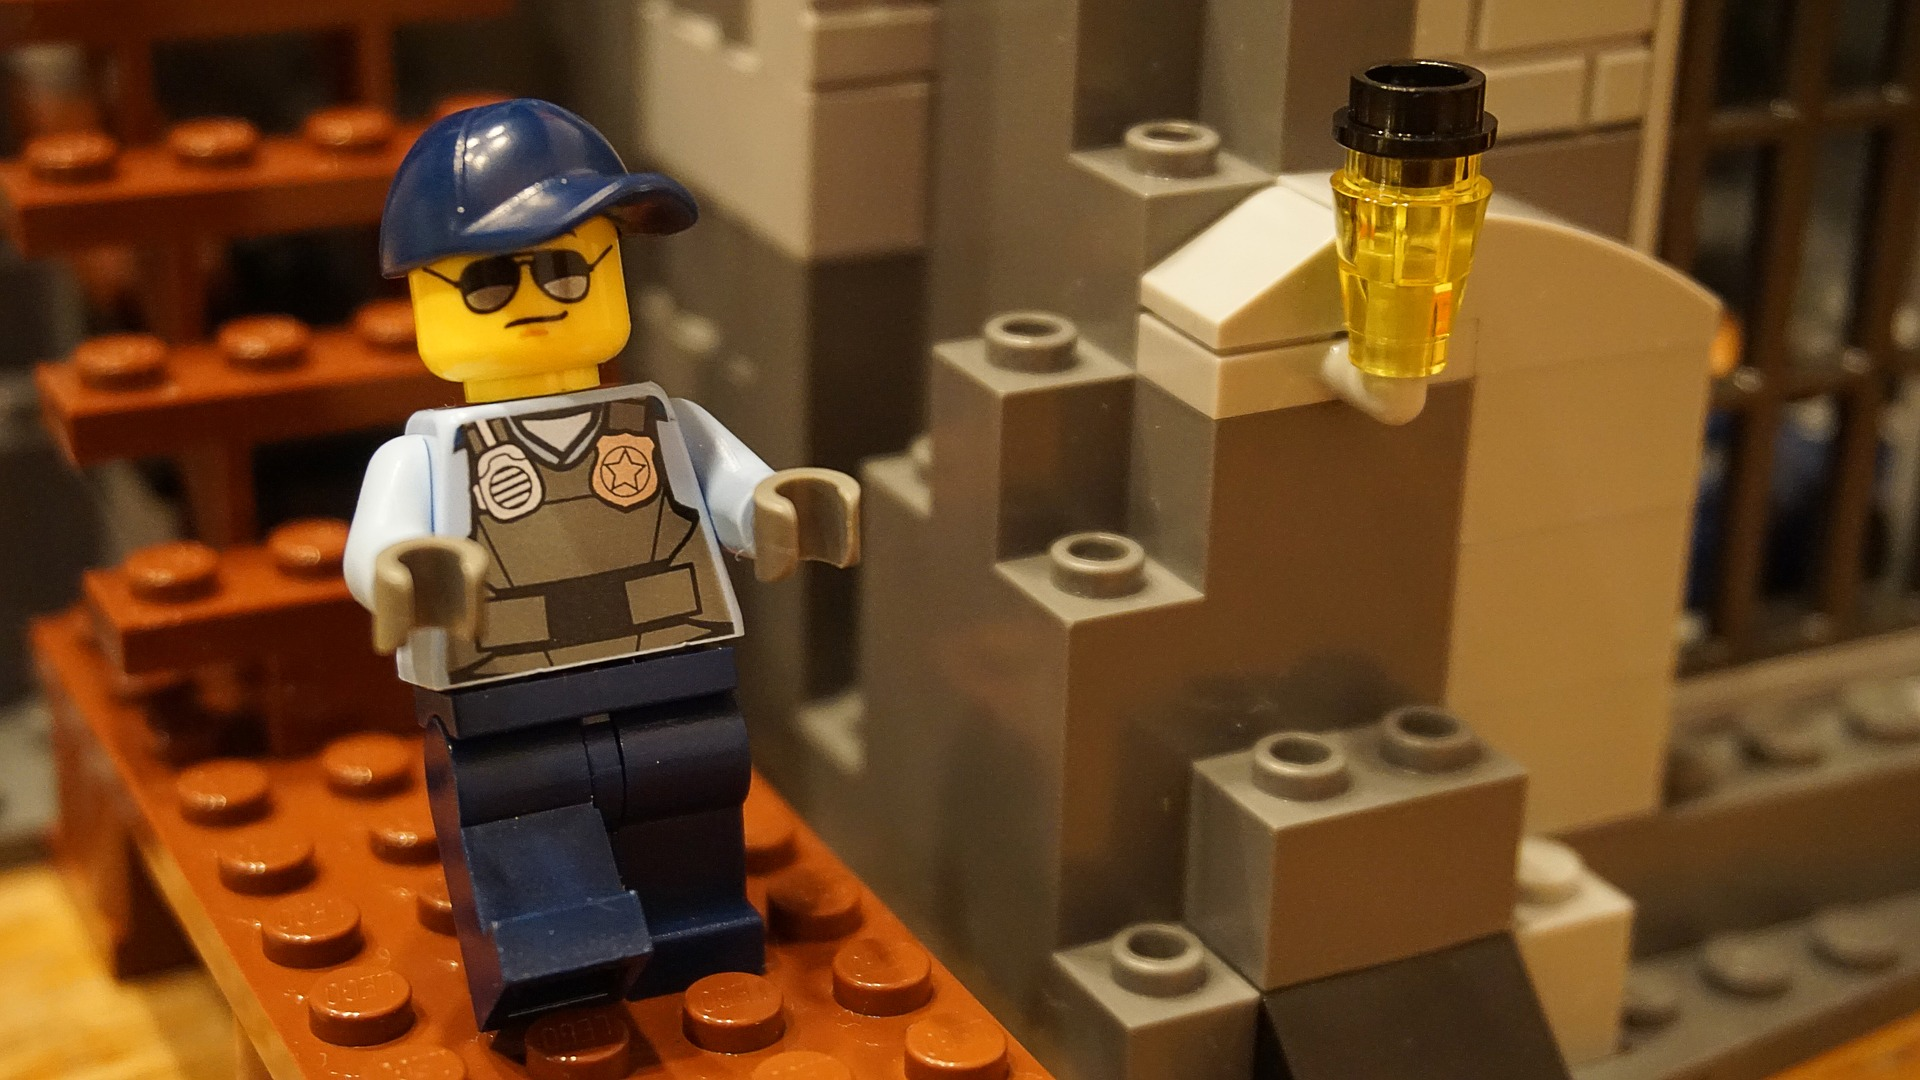
\includegraphics[keepaspectratio,width=.5\textwidth]{lego-ppr}}
\author[@2018 Prof. Jeferson Souza, MSc (jefecomp) - All rights reserved.]{
	\textcolor{blue}{Prof. Jeferson Souza, MSc.} \\[1mm] 
	\textcolor{blue}{\textit{{\footnotesize (jefecomp) }}}\\[1.5mm]
	 \underline{{\footnotesize jeferson.souza@udesc.br}}
	 \vspace*{1mm}
}
\institute[]{
\includegraphics[keepaspectratio,width=.5\textwidth]{template/logo_udesc_joinville_horizontal_assinatura}
}

\date{}

\titlegraphic{
\includegraphics[keepaspectratio,width=.2\textwidth]{template/logo_udesc_joinville_horizontal_assinatura}}

%%%%%%%%%%%%%%%%%%%%%%%%%%%%%%%%%%%%%%%%%%%%%%%%%%%%%%
%%%%%%%%%%%%%%%%%%%%%%%%%%%%%%%%%%%%%%%%%%%%%%%%%%%%%%
\begin{frame}[plain,noframenumbering]
\titlepage
\end{frame}

%%%%%%%%%%%%%%%%%%%%%%%%%%%%%%%%%%%%%%%%%%%%%%%%%%%%%%
%%%%%%%%%%%%%%%%%%%%%%%%%%%%%%%%%%%%%%%%%%%%%%%%%%%%%%
\section{Introdução}
\subsection{Introdução}
\begin{frame}{O que é um Requisito?}

\begin{alertblock}{\textbf{Requisito}}
Um requisito pode ser definido como uma necessidade, algo que é desejado e esperado. Exemplo: prestar atenção no professor é um requisito da disciplina Projeto de Programas (:-D).
\end{alertblock}

\end{frame}

\begin{frame}{Para que serve o Levantamento de Requisitos?}

\begin{alertblock}{\textbf{Finalidade}}
Descobrir e entender as reais necessidades do cliente, ou seja, o que o cliente realmente quer.
\end{alertblock}

\pause

\begin{alertblock}{\textbf{Ahh professor, isso é fácil....}}

Nãooooooooo! O levantamento de requisitos está longe de ser uma tarefa fácil...

\end{alertblock}

\pause 

\begin{alertblock}{\textbf{Por que?}}

Nem sempre o cliente sabe as suas reais necessidades, ou seja, não sabe muito bem o que quer.

\end{alertblock}

\end{frame}


\begin{frame}[allowframebreaks=.8]{O que esperar do Levantamento de Requisitos?}

\begin{itemize}
\itemsep 5mm

\item Compreender quais são as reais necessidades do cliente (O que o cliente realmente quer);

\item Compreender o negócio o qual a solução (produto/software) será desenvolvida;

\item Identificar pessoas que podem auxiliar no processo de especificação e entendimento dos requisitos;

\item Elaborar uma lista com os requisitos que descrevem as necessidades do cliente;

\item Identificar e remover ambiguidades entre os requisitos;

\item Criar casos de uso para auxiliar a identificação dos principais requisitos;

\item Em alguns casos, pode-se também produzir um protótipo simples para auxiliar a definição e o entendimento dos requisitos.
\end{itemize}

\end{frame}

%%%%%%%%%%%%%%%%%%%%%%%%%%%%%%%%%%%%%%%%%%%%%%%%%%%%%%
%%%%%%%%%%%%%%%%%%%%%%%%%%%%%%%%%%%%%%%%%%%%%%%%%%%%%%
\section{Dificuldades}
\subsection{Dificuldades}

\begin{frame}{Principais dificuldades}

\begin{itemize}
\itemsep 5mm

\item Definição de escopo;

\item Entendimento do problema/necessidade;

\item Mudanças.

\end{itemize}

\end{frame}

\begin{frame}{Definição de escopo}

\begin{alertblock}{\textbf{Problemas de escopo}}
Durante o levantamento de requisitos os limites da solução (produto/software) não ficam muito bem definidos, ou o cliente especifica detalhes técnicos que mais confundem do que ajudam a definir claramente os objetivos do sistema.
\end{alertblock}

\end{frame}

\begin{frame}{Entendimento do Problema/Necessidade}

\begin{alertblock}{\textbf{Entendimento}}
O cliente tem dificuldade para saber o que realmente quer, um baixo conhecimento do seu próprio negócio, e/ou problemas de comunicar suas necessidades. 
\end{alertblock}

\end{frame}

\begin{frame}{Mudanças}

\begin{alertblock}{\textbf{Ahhh a passagem do tempo....}}
Os requisitos podem mudar com o passar do tempo, e então atualizações precisam ser realizadas nos requisitos já definidos anteriormente.
\end{alertblock}

\end{frame}

%%%%%%%%%%%%%%%%%%%%%%%%%%%%%%%%%%%%%%%%%%%%%%%%%%%%%%
%%%%%%%%%%%%%%%%%%%%%%%%%%%%%%%%%%%%%%%%%%%%%%%%%%%%%%
\section{Início}
\subsection{Início}

\begin{frame}{Iniciar o Levantamento de Requisitos}

\begin{alertblock}{\textbf{O início}}

O método mais comum para iniciar o levantamento de requisitos é realizar uma reunião ou entrevista com o cliente. 

\end{alertblock}

\pause

\begin{alertblock}{\textbf{Dificuldades?}}
Sim, o início nunca é fácil!
\end{alertblock}

\end{frame}

\begin{frame}{Iniciar o Levantamento de Requisitos}

Iniciar o levantamento de requisitos passa por:

\begin{itemize}
\itemsep 5mm

\item Falta e dificuldade de comunicação entre as partes (cliente e equipe técnica);

\item Entendimentos divergentes do mesmo problema/domínio;

\item Nenhuma das partes sabe como e o que perguntar;

\item Expectativas podem ser diferentes (pelo menos no início).

\end{itemize}

\pause

\begin{alertblock}{\centering \textbf{Porém...}}

Ambas as partes (cliente e equipe técnica) tem o desejo que o relacionamento que começa a ser estabelecido seja bem sucedido.
\end{alertblock}

\end{frame}

\begin{frame}{Iniciar o Levantamento de Requisitos}

\begin{alertblock}{\centering E então, como começar?}
\end{alertblock}

\pause

Comece com perguntas mais genéricas, tais como: 

\begin{itemize}[<+->]
\itemsep 5mm

\item Quais serão os benefícios do software para a sua empresa?

\item Quem vai usar o software?

\end{itemize}

\pause

\begin{alertblock}{\centering \textbf{Qual o objetivo dessas perguntas?}}
Ganhar o entendimento do cliente, dos objetivos gerais, e dos benefícios que a solução deve fornecer.
\end{alertblock}

\end{frame}

\begin{frame} {Iniciar o Levantamento de Requisitos}

Na sequência, é necessário entender o problema e as expectativas do cliente a respeito do software. Para isso, faça perguntas tais como:

\begin{itemize}[<+->]
\itemsep 5mm

\item Que tipo de saída (resultado) você espera que o software forneça? Um gráfico? Uma tabela?

\item Qual são os principais problemas que o software poderá resolver? Melhorias de processo? Agilidade no acesso a informação?

\item Qual é o ambiente e qual o perfil das pessoas que utilizarão o software?

\end{itemize}

\end{frame}

\begin{frame}{Iniciar o Levantamento de Requisitos}

Por fim, é necessário identificar se as pessoas presentes na reunião são realmente quem devem responder todas as perguntas. Logo, o papel da equipe técnica é conduzir o foco da reunião:

\begin{itemize}[<+->]
\itemsep 5mm 

\item Existe mais alguma pessoa que deve ser envolvida no processo?

\item As respostas as minhas perguntas são oficiais, ou ainda precisam ser validadas?

\item Será que chegamos a uma visão geral e conjunta da solução?

\end{itemize}

\end{frame}

%%%%%%%%%%%%%%%%%%%%%%%%%%%%%%%%%%%%%%%%%%%%%%%%%%%%%%
%%%%%%%%%%%%%%%%%%%%%%%%%%%%%%%%%%%%%%%%%%%%%%%%%%%%%%
\section{Processo}
\subsection{Processo}

\begin{frame}{Trabalhar em Equipe Com o Cliente}

\begin{itemize}
\itemsep 5mm

\item Necessidade de quebrar a barreira que coloca o cliente em uma posição isolada, e com uma visão da solução que pode ser diferente da visão que se quer desenvolver;

\item Sessões de perguntas e respostas, juntamente com reuniões similares ao início do projeto não funcionam;

\item É necessário trabalhar em conjunto para refinar os requisitos.

\end{itemize}

\end{frame}

\begin{frame}{Aplicando a abordagem FAST}

O termo \textit{FAST} vem do inglês \textit{Facilitate Application Specification Techniques}, e descreve a criação de uma equipe em conjunto com o cliente para realizar o levantamento de requisitos de forma eficiente. A abordagem \textit{FAST} auxilia:

\begin{itemize}

\item Identificar o problema de forma eficiente;

\item Definir e propor aspectos da solução;

\item Estabelecer uma negociação dos requisitos e da solução;

\item Definir um conjunto preliminar de requisitos da solução de software que será implementada.

\end{itemize}

\end{frame}

\begin{frame}{Principais Características da \textit{FAST}}

\begin{itemize}
\itemsep 5mm

\item Reuniões em locais neutros (de preferência);

\item Estabelecimento de regras de preparação para os participantes;

\item Cada reunião tem uma agenda proposta que deve seguida, mas ao mesmo tempo deve permitir a exposição de idéias;

\item A existênca da figura de um ``mediador" que tem o controle da reunião;

\item Ata do que foi discutido e decidido na reunião.

\end{itemize}

\end{frame}

\begin{frame}{Pré-requisitos da \textit{FAST}}

Antes de iniciar a sequência de reuniões usando a abordagem \textit{FAST}, alguns pré-requisitos devem ser assegurados:

\begin{itemize}

\item Escopo e visão geral da solução bem definidos;

\item Especificação de um documento curto (1 ou 2 páginas) que descreve os objetivos, escopo, e a visão geral da solução (o que será feito).

\item Definição do mediador (cliente, engenheiro de software, analista de negócio, consultor externo);

 \item Definição de local, data e hora. 

\end{itemize}

\end{frame}

\begin{frame}{Pré-requisitos da \textit{FAST}}

Antes da primeira reunião cada participante deve fazer uma lista com os seguintes items:

\begin{itemize}
\itemsep 5mm

\item Aspectos do ambiente onde a solução será utilizada;

\item O que deve ser produzido pela solução;

\item Que tipo de recurso deve ser utilizado pela solução;

\item Recursos/serviços (processos ou funções) que manipulam os dados ou interagem com a solução;

\item Restrições em termos de custo, tamanho, regras de negócio, etc.

\end{itemize}

\end{frame}

\begin{frame}{Exemplo de Descrição de Solução}

\begin{alertblock}{\textbf {Exemplo~\cite{Pressman-2001}}}
Nossas pesquisas indicam que o mercado para sistema de vigilângia doméstica está crescendo a uma taxa de 40\% ao ano. Portanto, a idéia da empresa é entrar nesse mercado com a criação de um sistema de vigilância doméstica baseado em microprocesor que permita idealmente a proteção e o reconhecimento de um conjunto de incidentes indesejáveis tais como: entrada não-autorizada, fogo, alagamentos, entre outros. O produto, cujo o nome preliminar é \textit{SafeHome}, usará sensores apropriados para detectar cada incidente indesejado, poderá ser programado pelo próprio dono da propriedade, e telefonará para uma equipe de monitoramento (empresa de segurança) caso algum dos incidentes indevidos ocorra.
\end{alertblock}
\end{frame}

\begin{frame}{Exemplo:  Aspectos do Ambiente}

\begin{itemize}
\itemsep 5mm

\item Detectores de fumaça;

\item Sensores de portas e janelas;

\item Sensores de detecção de movimento;

\item Eventos (um sensor detecta algo e é ativado);

\item Painel de controle;

\item Entre outros.

\end{itemize}

\end{frame}

\begin{frame}{Exemplo: O que Deve Ser Produzido}

\begin{itemize}
\itemsep 5mm

\item Alerta telefônico;

\item Alarme sonoro;

\item Controle de incêndio;

\item Isolamento de área afetada.

\end{itemize}

\end{frame}

\begin{frame}{Exemplo: Recursos/Serviços}

\begin{itemize}
\itemsep 5mm

\item Configuração do alarme;

\item Programação do sistema (liga/desliga sensores, senha de acesso);

\item Monitoramento dos diferentes sensores;

\item Acionamento de portas corta fogo;

\item Chamada telefônica.

\end{itemize}

\end{frame}

\begin{frame}{Exemplo: Restrições}

\begin{itemize}
\itemsep 5mm

\item Custo de produção inferior a R\$200 (por exemplo);

\item Interface de utilização amigável (fácil de usar e intuitiva);

\item Interagir diretamente com sistema telefônico;

\item Incidente indesejável deve ser reconhecido dentro de 1 segundo;

\item Definir prioridade de eventos (fogo é mais prioritário que abertura de janela).

\end{itemize}

\end{frame}

\begin{frame}{Aspectos da primeira reunião}

\begin{itemize}
\itemsep 5mm

\item Discutir a necessidade e a justificativa da nova solução (todos devem concordar nesses pontos);

\item Apresentação das lista de items (aspectos, resultados esperados, recursos/serviços, restrições) de cada um dos participantes;

\item Criação de uma lista de items única pelo grupo de participantes.

\item divisão do grupo em pequenos grupos de trabalho que produzirão a especificação do sistema em pequenas partes (no caso de grupos de trabalho grandes).

\end{itemize}

\end{frame}

\begin{frame}{Aspectos das reuniões seguintes}

\begin{itemize}
\itemsep 5mm

\item Apresentação das especificações que forem sendo produzidas sobre a solução;

\item Alteração das especificações (inclusão, atualização, e remoção de items);


\end{itemize}

\pause

\begin{alertblock}{\centering \textcolor{red}{Importante!}}
Todos os aspectos da reunião devem ser coordenados pelo mediador.
\end{alertblock}

\end{frame}

%%%%%%%%%%%%%%%%%%%%%%%%%%%%%%%%%%%%%%%%%%%%%%%%%%%%%%
%%%%%%%%%%%%%%%%%%%%%%%%%%%%%%%%%%%%%%%%%%%%%%%%%%%%%%
\section{Classificação}
\subsection{Classificação}

\begin{frame}{Classificação dos Requisitos}

Os requisitos pode ser classificados em três categorias:

\begin{itemize}
\itemsep 5mm

\item Normal;

\item Esperado;

\item Diferencial.

\end{itemize}

\end{frame}

\begin{frame}{Requisitos Normais}

\begin{alertblock}{\textbf{Definição}}
Descrevem os objetivos que foram definidos juntamente com o cliente durante as reuniões.
\end{alertblock}

\pause

\begin{alertblock}{\centering \textcolor{red}{Importante!}}
A presença dos requisitos normais já deixa o cliente satisfeito. Exemplo: O sistema deve produzir relatórios com indicadores de custo de produção por hora, dia, e mês.
\end{alertblock}

\end{frame}

\begin{frame}{Requisitos Esperados}

\begin{alertblock}{\textbf{Definição}}
Descrevem os requisitos que são implícitos da solução (produto/software) a ser desenvolvido. Exemplo: o sistema deve fornecer resultados corretos.
\end{alertblock}

\pause

\begin{alertblock}{\centering \textcolor{red}{Importante!}}
A presença dos requisitos é fundamental para assegurar os requisitos normais, e o bom funcionamento da solução.
\end{alertblock}

\end{frame}

\begin{frame}{Requisitos Diferenciais}

\begin{alertblock}{\textbf{Definição}}
Descrevem caracteristicas que vão além da expectativa do cliente, e deixam o mesmo ainda mais satisfeito. Exemplo: o sistema deve fornecer uma planejamento de custos baseado no histórico de utilização do cliente.
\end{alertblock}

\pause

\begin{alertblock}{\centering \textcolor{red}{Importante!}}
A presença dos requisitos diferenciais permitem um aumento do valor agregado da solução.
\end{alertblock}

\end{frame}

%%%%%%%%%%%%%%%%%%%%%%%%%%%%%%%%%%%%%%%%%%%%%%%%%%%%%%
%%%%%%%%%%%%%%%%%%%%%%%%%%%%%%%%%%%%%%%%%%%%%%%%%%%%%%
\section{}

\begin{frame}[plain,allowframebreaks,noframenumbering]{Bibliografia}

\begin{thebibliography}{Pressman, 2001}

\bibitem[Pressman, 2001]{Pressman-2001}

Pressman, R.

\newblock{{\em ``Software Engineering: A Practioner's Approach"}. 4th edition. McGraw-Hill, 2001.}

\end{thebibliography}

\end{frame}

\begin{frame}[plain,noframenumbering]

\begin{center}

\includegraphics[keepaspectratio, width=.8\textwidth]{template/happycat-end}
\end{center}
\end{frame}

\end{document}